\documentclass[sigconf, anonymous]{acmart}



\usepackage{listings}



\newcommand{\FigHighLevel}{

\begin{figure}[ht]
    \centering
    % 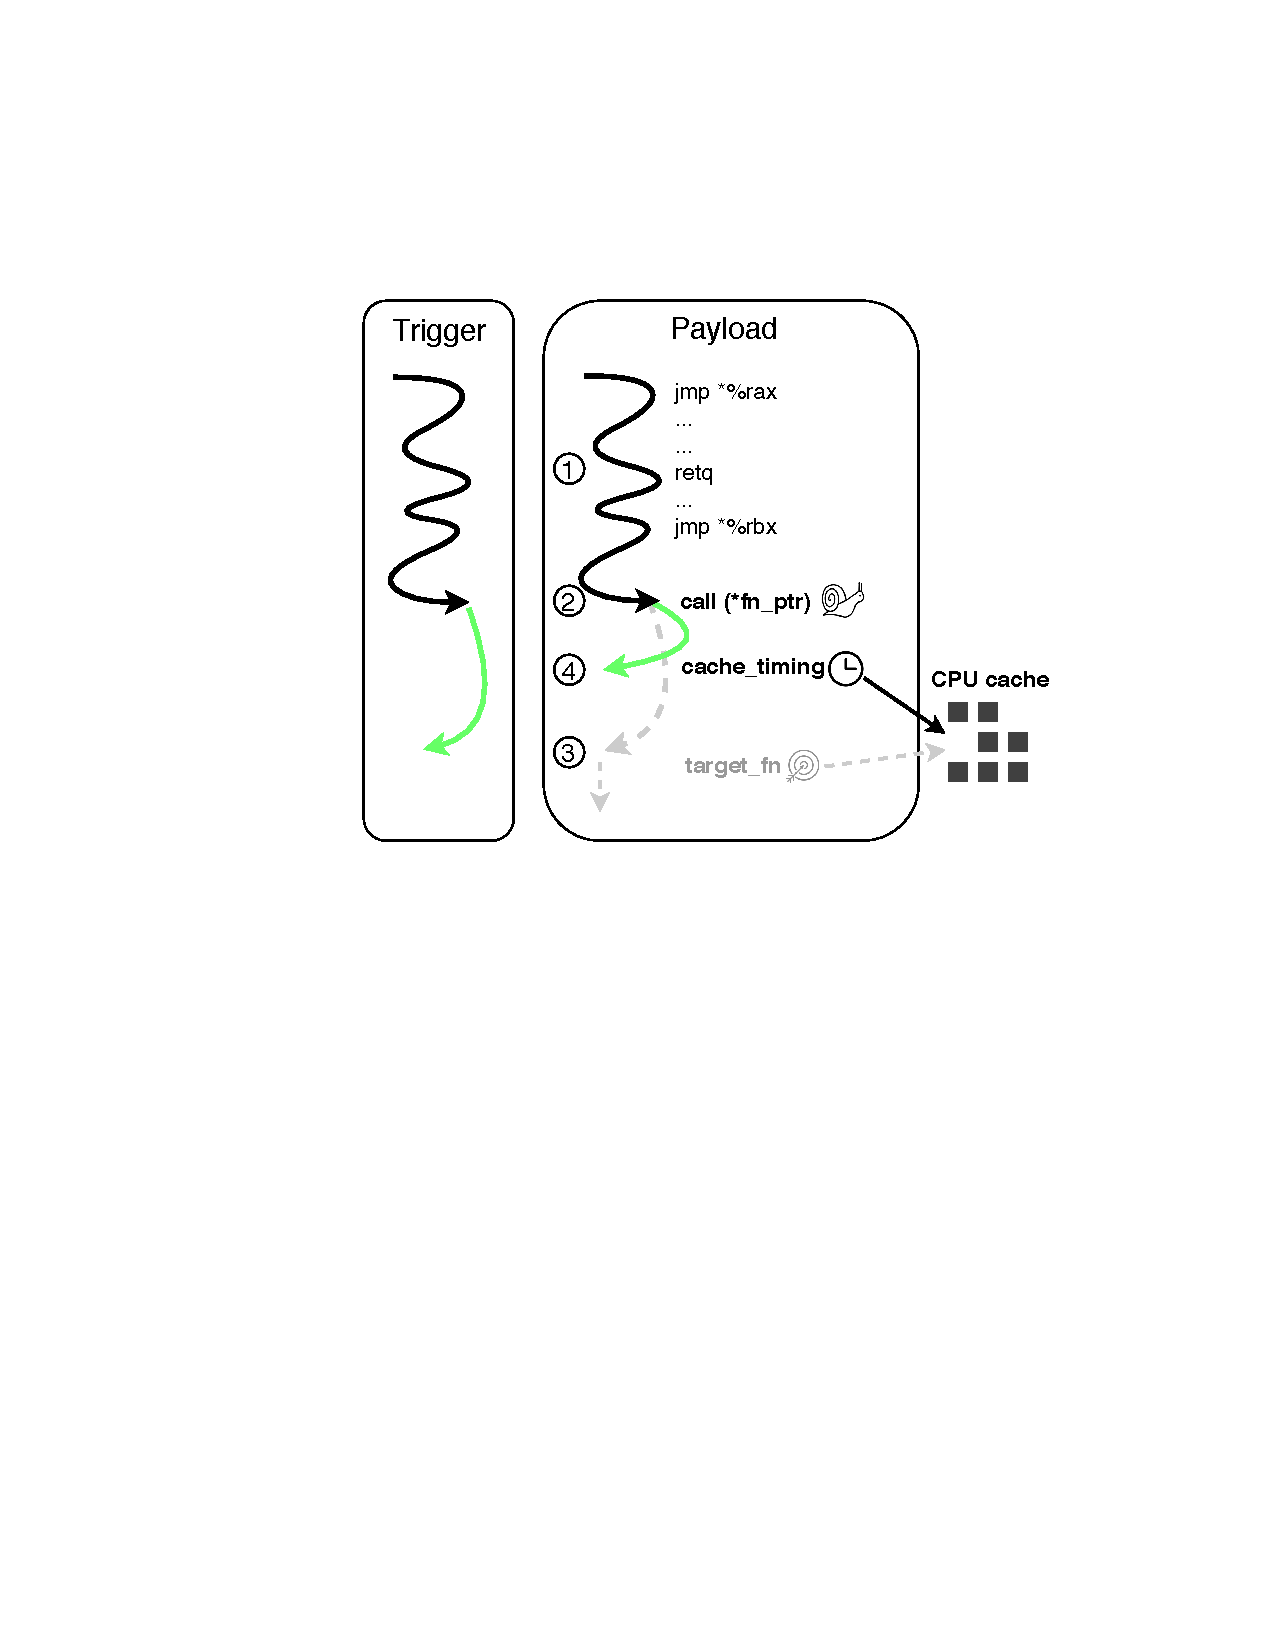
\includegraphics[clip, trim=6cm 13.5cm 3.8cm 5cm, width=0.9\linewidth]{figures/exspectre-high-level.pdf}
    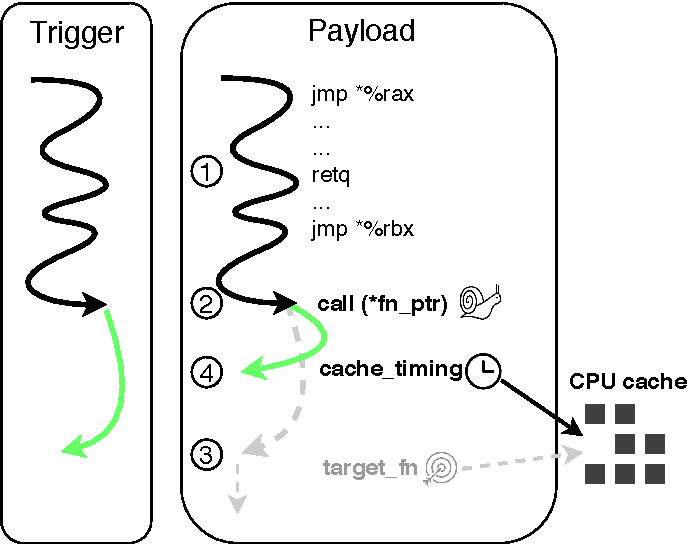
\includegraphics[width=0.9\linewidth]{figures/exspectre-high-level-trimmed.pdf}
    \caption{\textbf{Exspectre}\,---\, %
    1, 2, 3, 4...}

    \label{fig:high-level}

\end{figure}
}


\newcommand{\FigSpecMeasure}{
\begin{figure*}[t]
    \centering
        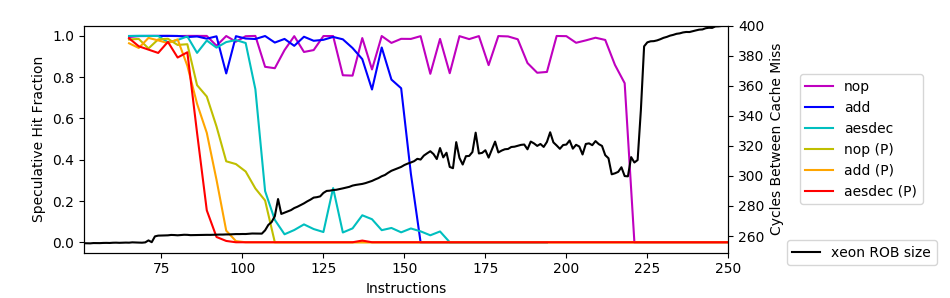
\includegraphics[width=0.9\textwidth]{figures/Speculative_measurements.png}
    \caption{The speculative primitive allows for a limited number of instructions
        to be completed speculatively, dependent on multiple factors. Trigger and 
        payload processes must share cpu resources as they must be performed on 
        the same hyperthread or associated parity hyperthreads. Processes on
        the parity hyperthreads (warm colors) denoted by (P) accomplish a 
        significantly lower number of instructions as compared with processes 
        on the same hyperthread (cool colors).}
    \label{fig:spec-capacity}
\end{figure*}
}


\newcommand{\FigCacheMiss}{
\begin{figure}[t]
    \centering
    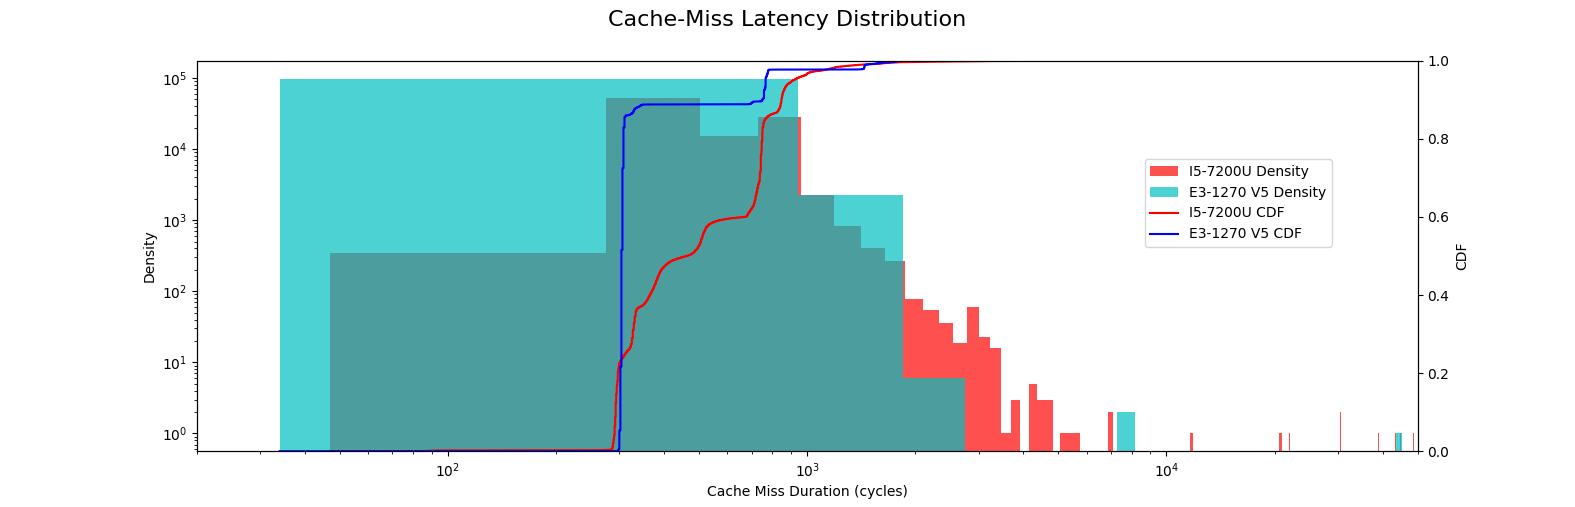
\includegraphics[width=0.5\textwidth]{figures/cache_miss_dist}
    \caption{Cache Hit/Miss Latency Distribution}
    \label{fig:cache-miss}
\end{figure}
}


\newcommand{\FigGeneralModel}{
\begin{figure}[t]
    \centering
        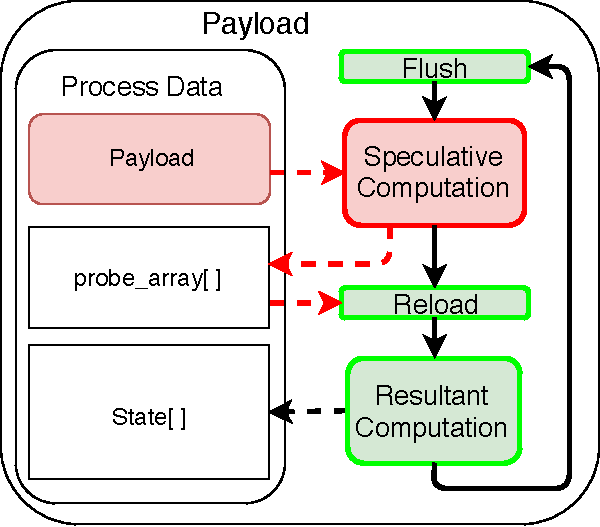
\includegraphics[width=0.4\textwidth]{figures/general_model.pdf}
    \caption{ General model of speculative computation within the Measure 
        process when triggered. \textit{Speculative Computation} has access
        to all variables which do not require a memory transaction within
        the current state of the process. The process can subsequently make
        \textit{Resultant Computations} based on the value returned from 
        \texttt{Flush+Reload} to update the state of the process. }
    \label{fig:general_model}
\end{figure}
}


\newcommand{\FigSpecBandwidth}{
\begin{figure}[t]
    \centering
        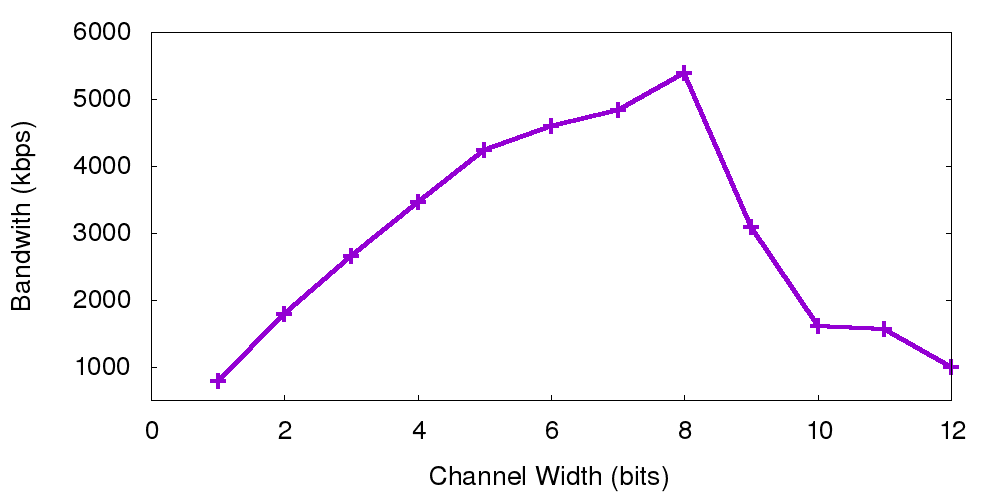
\includegraphics[width=0.5\textwidth]{figures/Speculative_bandwidth}
    \caption{Speculative Bandwidth - Using the speculative primitive 
        1KB of data can be decrypted and exfiltrated at a speed between 5 and 6 kbps
        from the speculative world. Varying the width of the channel 
        results in competing performance factors -- decreasing the 
        number of loops vs decreased size of the probe space.}
    \label{fig:spec_bandwidth}
\end{figure}
}



\newcommand{\FigSpasmModel}{
\begin{figure}[b]
    \centering
        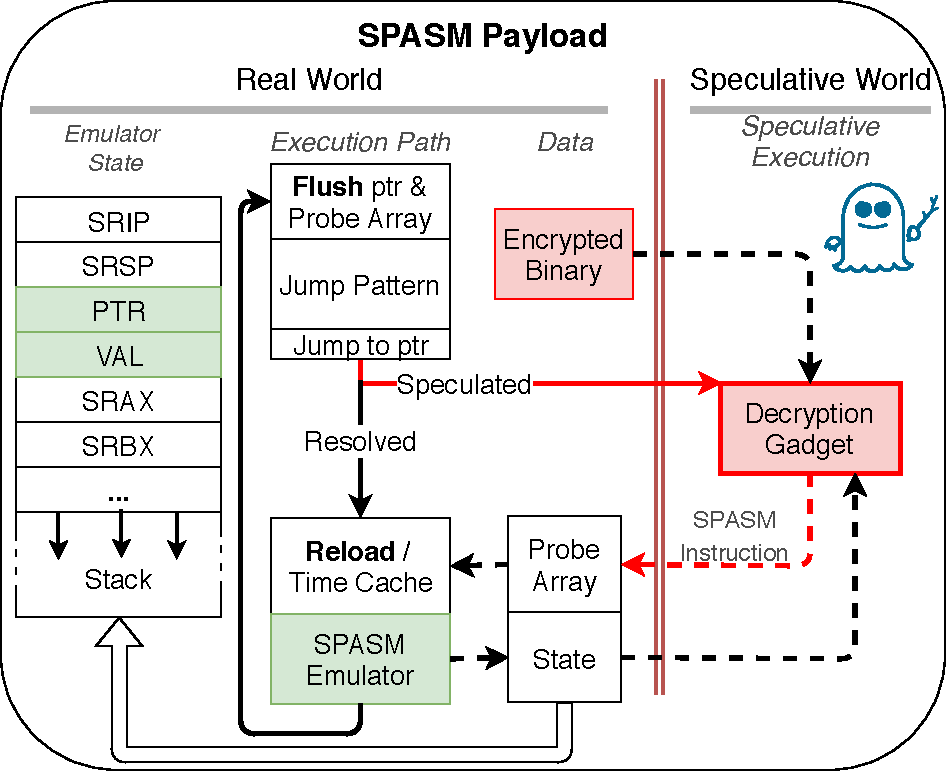
\includegraphics[width=0.5\textwidth]{figures/spasm_model.pdf}
    \caption{This model describes the VM control flow. An encrypted SPASM binary 
        stored in dead code or data accessible to \textit{Speculative Computation} 
        is decrypted  and then returned through the primitive. The SPASM 
        \textit{Resultant Computation} performs the SPASM emulation to update the 
        process state before the next instruction is decrypted.}
    \label{fig:spasm_model}
\end{figure}
}


\fancyhf{} % Remove fancy page headers 
\fancyhead[C]{Paper \#XXX} % TODO: replace 9999 with your paper number
\fancyfoot[C]{\thepage}

\setcopyright{none} % No copyright notice required for submissions
%\acmConference[Anonymous Submission to ACM CCS 2018]{ACM Conference on Computer and Communications Security}{Due 08 May 2018}{Toronto, Canada}
\acmYear{2017}

\settopmatter{printacmref=false, printccs=true, printfolios=true} % We want page numbers on submissions

%%\ccsPaper{9999} % TODO: replace with your paper number once obtained

\newcommand{\speculake}{Exspectre }


\begin{document}
\title{\speculake: Hiding Malware in Speculative Execution} % TODO: replace with your title

\begin{abstract}
Recently, the Spectre and Meltdown attacks have revealed serious vulnerabilities in modern CPU
designs, allowing an attacker to exfiltrate data from sensitive programs. These
vulnerabilities take advantage of speculative execution to coerce a processor to
perform computation that would otherwise not occur, leaking the resulting
information via side channels to an attacker.

In this paper, we extend these ideas in a different direction, and leverage speculative
execution in order to \emph{hide malware} from both static and dynamic analysis. Using this
technique, critical portions of a malicious program's computation can be shielded from view,
such that even a debugger following an instruction-level trace of the
program cannot tell how its results were computed.

We introduce \emph{\speculake}, which compiles arbitrary malicious code into a
seemingly-benign payload binary. When a separate trigger program performs a specific
pattern of indirect jumps, it (mis)trains the CPU's branch predictor. Subsequent
executions of the payload binary with similar jumps causes the CPU to mispredict its
branches and speculatively execute a malicious payload, which communicates
results back to the real world via side channels.

We study the extent and types of execution that can be performed in the
``speculative world'', and build tools that enable several computations to be
performed covertly. In particular, within speculative execution we are able to
decrypt memory using AES-NI instructions, and are able to interpret a custom
virtual machine language to perform arbitrary computation.
We also show how the trigger program
can be a pre-existing benign application already running on the system, and
demonstrate this concept with OpenSSL driven remotely by the attacker as our
trigger program.

Finally, we describe defenses, but in all honesty, you're probably not going to like
them.

We consider this to be a new thrust in attack vector research that harkens to work 
done on hardware red-pills and weird machines. We demonstrate that unintended 
functionality of architechture can be used to compose malicious programs with 
new and different properties. This technique poses novel and unique challenges for 
malware modeling efforts, as it forces an environment to either
faithfully reproduce all hardware behaviors, or overcome a much larger burden of 
reverse engineering. 


\end{abstract}

% TODO: replace this section with code generated by the tool at https://dl.acm.org/ccs.cfm

%\begin{CCSXML}
%<ccs2012>
%<concept>
%<concept_id>10002978.10003029.10011703</concept_id>
%<concept_desc>Security and privacy~Usability in security and privacy</concept_desc>
%<concept_significance>500</concept_significance>
%</concept>
%</ccs2012>
%\end{CCSXML}

%\ccsdesc{Security and privacy~Use https://dl.acm.org/ccs.cfm to generate actual concepts section for your paper}
% -- end of section to replace with generated code

\keywords{Malware; Covert Channel; Weird Machines; TK} % TODO: replace with your keywords

\maketitle

%%%%%%%%%%%%%%
\section{Introduction}


Modern CPU designs use speculative execution to maintain high instruction
throughput, with the goal of improving performance. In speculative execution,
CPUs execute likely future instructions while they wait for other slower
instructions to complete. When the CPU's guess of future instructions is correct, the
benefit is faster execution performance. When its guess is wrong, the CPU
simply discards the speculated results and continues executing along the true path.


Previously, it was assumed that speculative execution results
remain invisible if discarded, as careful CPU design maintains strict separation
between speculative results and updates to architectual state.
However, recent research has revealed side channels that violate this
separation, and researchers have demonstrated ways to exfiltrate results from speculative
computation. Most notably, the Spectre vulnerability allows attackers to leak
information from purposefully mis-speculated branches in a victim
process~\cite{spectre}. The Meltdown vulnerability uses speculative results of an
unauthorized memory read to sidestep page faults and leak protected memory from
the kernel~\cite{meltdown}. Both of these vulnerabilities focus on extracting
secret data from a process or operating system.

\medskip

In this paper, we explore another attack enabled by speculative execution:
\speculake, which \emph{hides computation} within
the ``speculative world''. Taking advantage of the CPU's speculation to secretly
perform computation,
we can produce binaries that thwart existing reverse engineering
techniques. Because the speculative parts of a program never ``truly'' execute,
we can hide program functionality in the unreachable dead code in a program.
Even a full instruction trace, captured by a hardware debugger or software
emulator, will be unable to capture the logic performed speculatively.
This technique could lead to sophisticated malware that hides its behavior
from both static and dynamic analysis.


Existing malware use several techniques to evade detection and
make it difficult for analysts to determine payload behavior of reported malware. 
For example, binary \emph{packers} or \emph{crypters} encode an executable payload as
data that must be ``unpacked'' at runtime, making it difficult to tell
statically what a program will do~\cite{malware-packers}. Malware may also use
\emph{triggers} that only run the payload when certain conditions are present, preventing
it from executing when it is inside an analysis sandbox or debugger.

However, with some effort, these existing techniques can be defeated. Analysts can use
dynamic execution to unpack malware and reveal its
behavior~\cite{balzarotti2010efficient}, and can use symbolic execution or code
coverage fuzzers to determine the inputs or triggers that will reveal malicious
behavior~\cite{moser2007exploring,schwartz2010all,wang2017angr,egele2012survey}.


\speculake provides a new technique to malware authors, allowing them to hide
program functionality in code that does not execute at runtime.


At a high level, \speculake consists of two parts: a payload program, and a
trigger program. When run by itself, the payload program executes a pattern of
indirect jumps and measures a cache side channel. While the trigger program is
not running, the payload program is effectively inactive (and may optionally do some
decoy operation). When the trigger program runs, it executes a similar pattern of
indirect jumps (with similar source and destination addresses as the payload
program), effectively training the CPU's branch predictor to the jump pattern
specified by the trigger program.

Importantly, the trigger program and payload
program's indirect jump patterns diverge on the destination of their final jumps.
However, because the trigger program has trained the CPU's branch predictor, the
CPU speculates that the payload program will continue following the pattern of
the trigger program, causing it to speculatively execute a
\emph{target function} in the payload program. We emphasize that this target
function is in a region that is neither read nor executed by the payload
program, and after the CPU discovers the mis-speculation in the payload program,
it will discard the results from the target function and continue executing from
the correct destination. However, the payload program has a limited speculative
window where it can perform computation in the target function, and can
communicate results back to the ``real world'' payload program via a cache side
channel.


While it's possible for the trigger and payload programs to be bundled in a
single program, an analyst aware of \speculake could easily find the target
function in the payload program based on the jump pattern in the trigger program.
However, if the trigger and payload are kept separate, the analyst has a much
harder job and must identify both.
Moreover, it is possible that the trigger program be a
seemingly-unrelated benign program already on the victim's computer. We
investigate using the OpenSSL library as a benign trigger
program in Section~\ref{sec:tk}. If the trigger program is another benign
program on the system, the analyst has the difficult task of identifying which
program, library, or even operating system component is responsible for training
the CPU's branch predictor, and finding the specific set of jumps that occur at
runtime. To make matters worse, the payload program can include dummy jump
patterns that are effectively dead ends for the analyst, as they do not
ultimately call the target function speculatively.


Simulating or modelling the speculative execution path is a difficult task for a
program analyst hoping to reverse engineer an \speculake binary. First, the
analyst must reverse engineer and accurately model the closed-source proprietary
components of the target CPU, including the branch predictor, cache hierarchy,
out-of-order execution, and hyperthreading. In contrast, the \speculake
author only has to use a partial model of these components and produce binaries
that take advantage of them, while the analyst's model must be complete to
capture all potential \speculake uses. Second, the analyst must run all
potential trigger programs through the simulator, including benign programs with
realistic inputs. Both of these contribute to a time-consuming and expensive
endeavor for would-be analysts.

% Results summary
In order to study the potential of \speculake, we implement several example
payload programs and evaluate their performance.
We find that the speculative window is limited mainly by the reorder buffer
size, and confirm that we are able to execute between 100 and 200 instructions
speculatively on modern Intel CPUs. While brief, we are able to perform
execution in short steps, communicating intermediate results back to the ``real
world'' part of the payload program. Using this technique,
we demonstrate implementing a universal Turing machine
(demonstrating arbitrary computation), a custom instruction set architecture
that fits within the constraints of speculative execution, and show
the ability to perform AES decryption
of a payload via AES encrypt/decrypt instructions. 

Using these building blocks, we demonstrate the practicality of hiding arbitrary
computation by decrypting an AES-encrypted ARM binary in the speculative world
one instruction at a time, returning the decrypted next instruction to the real
world part of the payload program, which updates a virtual machine. We show that
we are able to decrypt and process approximately 25 instructions per second.


% contributions?
% - explore the limits of speculative execution
% - propose novel concept of hiding computation in speculative execution
% - implement example applications using this concept, including decrypting
%   data speculatively
% - demonstrate using benign program (openssl) as trigger
% - identify defenses and discuss ways to counter them





% TODO: we don't talk at all about how an analyst might try to enumerate
% the potential entry points to the speculative world, and how that can be
% made difficult




%%%%%%%%%%%%%%
\section{Background}
Modern CPU designs employ a wide range of tricks in order to maximize
performance. In this section, we provide preliminary background as they are
relevant to our system, as well as a brief summary of the Spectre vulnerability.

\subsection{Out-of-Order Execution}
Many CPUs attempt to keep the pipeline full by executing instructions \emph{out of
order}, with the CPU allowing future instructions to be worked on and executed
while it waits for slower or stalled instructions to complete. To maintain
correctness and the original (Von Neumann) ordering, instructions are tracked in
a \emph{reorder buffer} (ROB), which keeps the order of instructions as they are
worked on out of order. Instructions are \emph{retired} from the ROB when
they are completed and there are no previous instructions that have yet to
retire. Upon retiring, an instruction's results are committed to the architectural
state of the CPU. Thus, the ROB ensures that the program (or debugger) view
of the CPU state always updates in program execution order, despite out of order
execution.

\subsection{Speculative Execution}

CPUs also attempt to keep their pipeline full by predicting the path of
execution. For example, a program may contain a branch that depends on a result
from a prior slow instruction. Rather than wait for the result, the CPU can
\emph{speculatively execute} instructions down one of the paths of a branch,
storing the results of the speculative instructions in the ROB.
If the guess of the branch target turns out to be correct, the CPU can quickly
retire all the instructions it has speculatively executed while waiting. If the
guess is incorrect, the CPU must discard the
(incorrectly) speculated instructions from the ROB, and continue executing from the
correct branch target.


\subsection{Branch Prediction}
When a CPU mispredicts a branch, the speculative execution results are
discarded, costing the CPU several cycles as the pipeline is flushed. To
minimize this, CPUs employ \emph{branch predictors} that attempt to guess the
path of execution. Branch predictors maintain a short history of previous
branch targets for a particular branch (e.g. whether a certain branch is
frequently taken or not taken), and use
this to inform the CPU's guess for speculative execution.

There are two kinds of branches a CPU handles: \emph{direct} and
\emph{indirect}. A \emph{direct} branch may either jump to a provided address or
continue executing straight through depending on the state of the CPU (e.g. condition
registers). While there are only two potential statically-known targets for a direct
branch, the CPU may not know if the branch is taken or not until preceding
instructions retire. An \emph{indirect} branch is always taken, but its address
is determined by the value of a register or memory address. Direct branches are
typically used for control flow such as \texttt{if} or
\texttt{for}/\texttt{while} statements, while indirect branches are used for
function pointers, class methods, or case statements.


%- BHB, BTB

\subsection{Spectre}

In early 2018, researchers revealed the Spectre vulnerability, which allows an
attacker to leak information from a victim program~\cite{specte}. Spectre uses
the fact that speculative execution can influence system state via side
channel. In Spectre, an attacker mistrains the branch predictor of a CPU running
a victim program by providing inputs to it. Once mistrained, the attacker then
sends a new input that will cause a different in-order execution path. However,
because the CPU's branch predictor has been mistrained, it will still
speculatively execute the previous path.

Consider the following code snippet from the Spectre
paper~\cite{spectre}:

\begin{lstlisting}
    if (x < array1_size)
        y = array2[array1[x] * 256];
\end{lstlisting}

The \texttt{if} statement correctly protects an out-of-bounds reads from \texttt{array1}.
But if the branch predictor makes an incorrect guess on the branch's direction
and speculatively executes inside the \texttt{if} statement, it may
cause a read beyond the boundary of \texttt{array1}. The result of this will
then (speculatively) be multiplied by 256 and used as an index into
\texttt{array2}. Although the CPU will not commit
the speculative update to \texttt{y}, it will still issue a memory read to
\texttt{array2[array1[x]*256]}, which will be cached. Importantly, even after
the CPU realizes the branch misprediction, it does not rollback the
state of the cache, as this does not directly influence program correctness.
However, the set of cached values is observable to the program via a
side-channel: by timing reads to \texttt{array2[i]}, the fastest read will
reveal the speculative value of \texttt{array1[x]*256}, for any value of
\texttt{x}. An attacker that is able to perform such a side-channel inference on
the cache can learn the speculative result of an out-of-bounds read from
\texttt{array1}.


Spectre can also be applied to indirect branches. Branch predictors use the
history of previous branches to predict the destination of an indirect jump when
the destination is not yet known. For direct branches, only one of two
destinations (taken or not taken) are possible to speculatively execute. But for
indirect branches, a mistrained branch predictor can potentially be coerced into
speculatively executing from \emph{any} target instruction in the binary.

We take advantage of the behavior of indirect branch prediction to hide the
location of our speculative computation.
%TODO more on why this is crucial...

%%%%%%%%%%%%%%
\section{Architecture}


\speculake malware is comprised of two independent programs: a payload program, and a
trigger program. Both are installed on the victim's computer (e.g. via trojan, remote
exploit, or phishing), and must run simultaenously on the same physical CPU. We
note that the constraint of running programs on the same CPU is not a signifcant
burden: \texttt{taskset} can be used to limit a process to a core, or if not
available, the attacker can simply run multiple copies of the trigger or payload
program to coerce the OS scheduler to assign a payload/trigger pair to the same
core.

At a high level, the trigger program performs a series of indirect jumps in a
loop, training the branch predictor to this pattern. Meanwhile, the
payload program performs a subset of this jump pattern, then forces the CPU to
speculate by stalling the resolution of an indirect branch via a slow memory
read. The CPU will (mistakenly) predict the jump to follow the pattern performed
by the trigger program, and speculatively execute that destination in the
payload program.

\subsection{Indirect jumps}

Indirect branch predictors allow the CPU to predict the destination address of a
branch based solely off its source address and a brief history of previous
branch sources and destinations. While the inner-working details of modern CPU
branch predictors are proprietary, it is possible to reverse engineer parts of
their behavior, which we do in \speculake.

We created a simple trigger program that performs a series of 32 indirect jumps,
using the \texttt{jmpq *\%rax} instruction. Between each jump, we increment
\texttt{\%rax} to account for the number of bytes between jumps. For the last
jump, we load a function pointer into \texttt{\%rax} and do a final indirect
jump using \texttt{callq \%rax}.


In our payload program, we first perform the same 32 indirect jumps. We ensure
the source address of these jumps is the same as in the trigger program by
manually defining their containing function at a fixed address inside a linker
script. We also do the final indirect call to a function pointer, but with two
differences. First, the destination of the function pointer is a different
address, and second, the location of the function pointer in memory is uncached.
This forces the CPU to predict the destination of the indirect call, which it
predicts to be the destination of the function pointer in trigger program. In
the payload program, we purposefully place code at this address which acts as
the \emph{speculative entry point}. Even though the in-order execution of
payload program never executes or even reads from this address, the CPU will
briefly execute instructions there speculatively.

Eventually, the dereference of the uncached function pointer in payload program
will be resolved, and the CPU will recognize it has incorrectly predicted the
destination of its \texttt{callq} instruction. The results from the speculative
entry point instructions will be discarded, and the CPU will continue executing
from the correct destination. However, as the speculative code changes what is
loaded into the cache based on its results, it can covertly communicate its
results to the ``real world'' program.


TODO: Note that returns can also be indirect jumps, and rets/jmpq can be mixed
to a certain extent...need to document/quantify how much mixing can be done
still.


\subsection{Limits of Speculative Execution}
We performed several experiments to investigate how much computation can be done
speculatively. We performed these experiments on an Intel~(TODO: Jack fill in).
TODO: Jack describe experiment and results:

- Experiment w/ graph of number of instructions
- Limitation is in the ROB (cite other work that supports this)

\subsection{Speculative Primitive}

We summarize our findings into a \emph{speculative primitive}, which allows us to
speculatively (and covertly) perform approximately TK:150 arbitrary
instructions, and communicate a short (e.g. single byte) result to the real
world via a cache side channel. These speculative instructions are able to read
from any real-world memory or registers, but they cannot perform updates or
writes directly. To update memory, the speculative instructions must communicate
to the real world through a cache side channel.

We note a performance tradeoff between the size of communication (e.g. 4 bits vs 8
bits) and the time it takes the real world to recover the result from the side
channel. Using Prime+Probe~\cite{prime-probe} as our cache side channel,
recovering the result requires accessing all elements in an array exponential in
the size of the result (e.g. $2^8$ array reads to recover an 8-bit result). 
Therefore, there is a
performance advantage for keeping the size of the result small, and communicating
out small pieces of information that are aggregated by the real world.


%%%%%%%%%%%%%%
\section{Application Payloads}

While the amount of computation done in a single speculative execution is small,
we demonstrate several applications that can take advantage of multiple
speculative runs to carry out computation.

As a first step, we observe that this primitive can be used to trivially
implement a finite state machine: any logic can be done in the speculative
world, while
updates to the state are communicated to the real world where they are stored.
On the next run of the speculative instructions, they read from the real world
state (and other inputs), compute any state transitions, and communicate the
result. In this mode, the state is maintained by the real world, while updates
are controlled by code executed speculatively.



\subsection{Turing Machine}
- Arbitrary computation

\subsection{Unpacking and Decryption}
- AES instructions

\subsection{Virtual Machines}
- SPASM


%%%%%%%%%%%%%%
\section{Trigger Programs}
Easy answer: custom program that mistrains branch predictor

\subsection{Benign Triggers}
Could also be any program on the system, and potentially remote!


\subsection{Complex Triggers}
When considering packers and crypters used in modern malware it is not uncommon to see 
a malicious sample packed using multiple stages with different unpacking conditions. 
Whether that be red pills, or environent checks, or network triggers, the reliance is on
complexity to fool any reverse engineer out of finding the correct conditions to 
release the full payload.

Similarly \speculake can be instrumented to use more than one trigger. Multiple stages 
can be designed used any combination of crafted or benign trigger programs. Only when all
stages have been run to completion in order will the malicious payload be revealed.  
In conjunction with this each stage cna use a randomized ISA to a common emulator, or 
they can use differnt emulators all together. 

Alternatively each stage could be used to decrypt the next AES key-schedule to decrypt 
a subsequent layer. Using this model we can instrument \speculake malware as a crypter 
with the keys hidden in data or dead code which static and dynamic reverse engineering 
methods will overlook. 


%%%%%%%%%%%%%%
\section{Implementation and Evaluation}

\subsection{Turing Machine}

\subsection{AES Decryption}

\subsection{Virtual Machine}

\subsection{OpenSSL Trigger}


%%%%%%%%%%%%%%
\section{Discussion}


\subsection{Defenses}


\subsection{Future Work}





%%%%%%%%%%%%%%
\section{Related Work}


%%%%%%%%%%%%%%
\section{Conclusion}


\bibliographystyle{ACM-Reference-Format}
\bibliography{paper}

\end{document}
